\newpage
\chapter{Физический смысл волновой функции в квантовой механике}
 
\begin{wrapfigure}[12]{r}{0.4\linewidth} 
\vspace{-2ex}
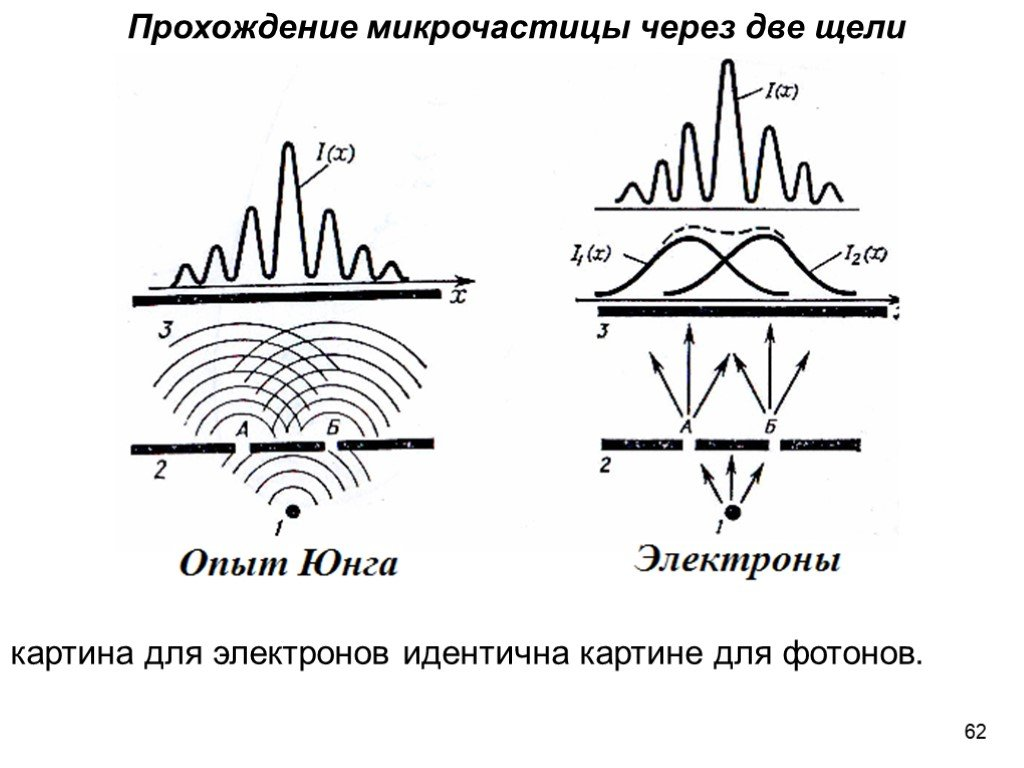
\includegraphics[width=0.9\linewidth]{pictures/4.2.jpg}
\caption{Схема эксперимента}
\end{wrapfigure}
\par Проведем мысленный эксперимент: пусть есть два экрана, первый из которых имеет два отверстия. Если же разместить перед экранами источник света, мы увидим ожидаемую интерференционную картинку, даже если закроем одно из отверстий. Заменим теперь источник света на источник электронов и зафиксируем наблюдения: если отверстия закрывать по очереди и посмотреть, какая картина будет суммарной, то получится совсем другой результат. Вывод: в некотором смысле частицы ведут себя точно так же, как волны, но вне зависимости от того, один электрон полетит или сразу пучок, при помещении лампочки перед экранами, картинка полностью пропадает. 
\par Пусть летит 1 электрон. Но интерференция не имеет место в данном случае, получается крайне идиотская ситуация - один и тот же электрон идет и через 1ое отверстие, и через второе сразу. Поставим еще лампочку перед 2 экраном - картинка пропадет совсем, даже если "стрелять" по одному электрону. Лампочка здесь играет роль некого источника ЭМ излучения, она позволяет увидеть (значит, измерить) рассеянное излучение - рассеяние частицы, но ведь выяснять уже нечего, т.к. картинки нет.
\par Значит, мы должны строить описание в терминах некой функции распределения $P(\vec{r})$, т. ч. интеграл по объему даст вероятность увидеть эту частицу в данном объеме. В оптике или волновой теории необходимо описание в терминах амплитуды и фазы волны, значит, требуется некая комплексная функция $ \psi (\vec{r}, t)$ и уравнение на нее. Знаем, что $|\psi (\vec{r}, t)|^2 d^3r$ может представлять собой вероятность (это действительная величина), так же $\psi$ предполагает взаимодействие с классическим прибором для понимания определения этой функции - \textit{волновой функции (комплексной амплитуды)}. Другими словами, посмотреть на электрон мы не можем, т.к. при отсутствии измерений нет и явлений, а при измерении прибором состояние сразу меняется. (О проблеме квантово-механического описания лучше не задумываться)
\par Пусть движение электрона через 1 отверстие описывает комплексная амплитуда $\psi _1$, а через второй - $\psi _2$ (хотя на самом деле стоит вводить целое множество, поговорим хотя бы про 2). Классические пути при столкновении с экраном интерферируют, на последнем экране видим фактически их сумму $c_1 \psi _1 + c_2 \psi _2 $, тогда взяв $ |c_1 \psi _1 + c_2 \psi _2 |^2$, получим распределение. Фазы комплексных функций будут зависеть от конкретных точек наблюдений. Анализируя эксперимент, мы должны складывать не вероятности прохождения, а комплексные амплитуды.
\par
\par В классической механике движение происходит по траектории, отвечающей минимуму функционала действия, а квантомеханическая частица может двигаться по различным траекториям (все они равновероятны), причем одновременно. В пустом пространстве (без экранов и отверстий) все так же. Частица идет сразу по всем траекториям, каждой из которых соотвествует некая $\psi$, результатом брать сумму всех таких пси по модулю в квадрате. В реальности частиц множество, как все устроено, если $\psi (\vec{r_1}, \vec{r_2}) $?
\par
\begin{wrapfigure}[12]{l}{0.3\linewidth} 
\vspace{-2ex}
\centering
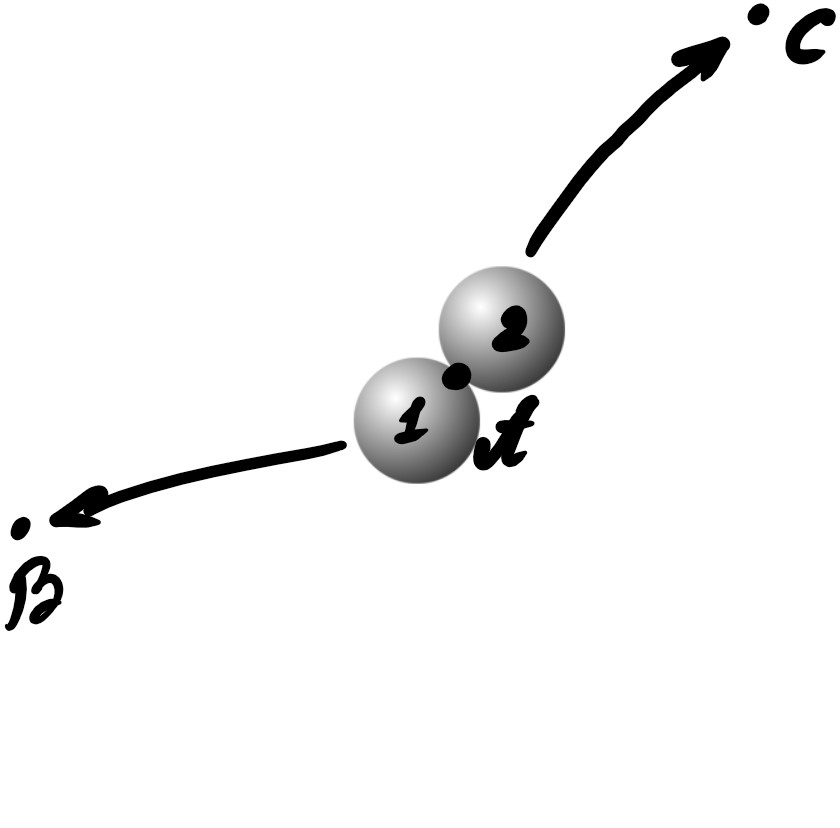
\includegraphics[width=0.8\linewidth]{pictures/5.2.jpg}
\caption{Иллюстрация к тексту}
\end{wrapfigure}
\par Практически постулат: пока частицы не взаимодействуют, можем искать волновую функцию как $ \psi _1 (\vec{r_1}) \cdot \psi _2 (\vec{r_2})$. Это автоматически означает, что  в уравнениях эти частицы подразумевают разделение переменных в таком пределе, т.е. они должны быть линейные. Допустим, в точке А было определенное состояние двух квантовомеханических частиц, их отпустили, частицы разлетелись далеко друг от друга. Проводя измерения в точке В, мы одновременно определим состояние $2^{ой}$ частицы в т. С, т.к. $\psi$ - общая.
\par Такая трактовка означает, что имеет место коллосальная степень нелокальности. При таком взгляде на вещи скорость света - не предел, но если мы измеряем что-то реальное, то расчеты дадут разумный результат, т.е. в ответах подобных пародоксов не возникает. 